% =============================================================================
% File        : presentation.tex
% Project     : The Knowledge Lifecycle of Large Language Models
% Purpose     : Conference deck. Branded with the five lifecycle colors used by
%               the paper, the poster, the repository, and the live demo.
% Authors     : Amey Thakur, Sarvesh Talele
% Repository  : https://github.com/Amey-Thakur/LLM-KNOWLEDGE-LIFECYCLE
% License     : CC BY 4.0
% =============================================================================
%
% Every slide carries speaker notes. Compile as-is for the projected deck; add
% the "notes=show" class option to print the notes alongside for rehearsal.
%
% Timing: 18 slides, paced for a 20-minute talk with 5 minutes of questions.

\documentclass[aspectratio=169]{beamer}

\usepackage{booktabs}
\usepackage{amsmath}
\usepackage{amssymb}
\usepackage{tikz}
\usetikzlibrary{arrows.meta, positioning, calc, fit, backgrounds}
\usepackage{hyperref}  % every URL in the deck is clickable in the PDF

% --- the five lifecycle colors, identical across every surface ---------------
\definecolor{acquire} {HTML}{4A7FD4}
\definecolor{store}   {HTML}{2A9D8F}
\definecolor{retrieve}{HTML}{E08A2E}
\definecolor{update}  {HTML}{D05353}
\definecolor{forget}  {HTML}{8F5FB8}
\definecolor{ink}     {HTML}{1A1A1C}
\definecolor{muted}   {HTML}{6C6C78}
\definecolor{rule}    {HTML}{DEDEE4}
\definecolor{ok}      {HTML}{2E7D32}

% --- a restrained theme: no shadows, no navigation clutter -------------------
\usetheme{default}
\usecolortheme{default}
\setbeamertemplate{navigation symbols}{}
\setbeamercolor{structure}{fg=acquire}
\setbeamercolor{frametitle}{fg=ink}
\setbeamercolor{normal text}{fg=ink}
\setbeamerfont{frametitle}{size=\Large, series=\bfseries}

% Beamer's default puts the frame title 9.65 pt down a 255 pt slide, against the
% colour band along the top edge. This template states the space above and below
% outright, so every slide carries the same 24 pt of air under the band.
\setbeamertemplate{frametitle}{%
  \vspace{16pt}%
  \usebeamerfont{frametitle}\usebeamercolor[fg]{frametitle}%
  \insertframetitle\par
  \vspace{6pt}%
}

\setbeamertemplate{itemize item}{\color{muted}\textbullet}
\setbeamertemplate{itemize subitem}{\color{muted}--}
\setbeamertemplate{caption}{\insertcaption}

% The five-stage band appears on every slide, so the deck is identifiable from
% any single slide photographed out of context.
\setbeamertemplate{background}{%
  \begin{tikzpicture}[remember picture, overlay]
    \foreach \c [count=\i from 0] in {acquire, store, retrieve, update, forget}
      \fill[\c] ($(current page.north west) + (\i*0.2\paperwidth, 0)$)
             rectangle ++(0.2\paperwidth, -0.055cm);
  \end{tikzpicture}%
}

\setbeamertemplate{footline}{%
  \hspace{0.6cm}\color{muted}\scriptsize
  Probability Is Not an Answer
  \hfill Thakur and Talele\hspace{0.4cm}\insertframenumber\hspace{0.6cm}\vspace{0.25cm}%
}

% A reusable author strip, so the title and closing slides cannot drift apart.
\newcommand{\authorstrip}[4]{%
  \begin{tikzpicture}
    \begin{scope}\clip (0,0) circle (#1);
      \node at (0,0) {
\includegraphics[width=2*#1]{amey-thakur.jpg}};\end{scope}
    \draw[rule, line width=1pt] (0,0) circle (#1);
    \node[below, font=#3\bfseries] at (0,-#1-0.15) {Amey Thakur};
    \node[below, font=\tiny, text=muted] at (0,-#1-0.55) {#2};
    \begin{scope}\clip (#4,0) circle (#1);
      \node at (#4,0) {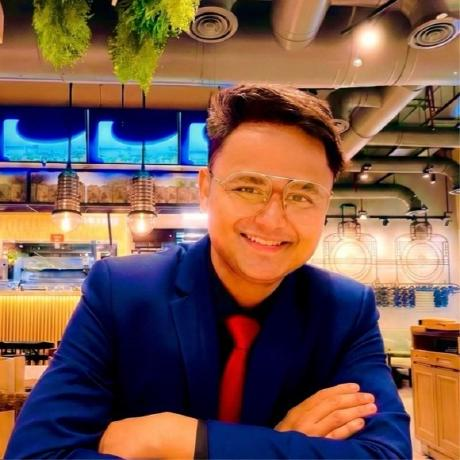
\includegraphics[width=2*#1]{sarvesh-talele.jpg}};\end{scope}
    \draw[rule, line width=1pt] (#4,0) circle (#1);
    \node[below, font=#3\bfseries] at (#4,-#1-0.15) {Sarvesh Talele};
    \node[below, font=\tiny, text=muted] at (#4,-#1-0.55) {\ifnum\pdfstrcmp{#2}{Toronto, Canada}=0 Mumbai, India\else talelesarvesh@gmail.com\fi};
  \end{tikzpicture}%
}

\hypersetup{colorlinks=true, urlcolor=acquire, linkcolor=acquire}

\title{Probability Is Not an Answer: Knowledge Conflict, Read at the Rank}
\author{Amey Thakur \and Sarvesh Talele}
\date{2026}

\begin{document}

% ============================== 1. TITLE =====================================
\begin{frame}[plain]
  \vspace{0.3cm}
  \begin{center}
    {\LARGE\bfseries Probability Is Not an Answer}\\[2mm]
    {\LARGE\bfseries Knowledge Conflict, Read at the Rank}\\[5mm]
    {\color{muted}\small A model holds two memories. Which one comes out is not a question of size.}\\[7mm]

    
\begin{tikzpicture}
      \foreach \c/\n [count=\i from 0] in
        {acquire/Acquire, store/Store, retrieve/Retrieve, update/Update, forget/Forget}
        \node[fill=\c, text=white, font=\footnotesize\bfseries, rounded corners=2pt,
              minimum width=2.1cm, minimum height=0.62cm] at (\i*2.3, 0) {\n};
    \end{tikzpicture}\\[9mm]

    \begin{tikzpicture}
      \begin{scope}\clip (0,0) circle (0.95cm);
        \node at (0,0) {
\includegraphics[width=1.9cm]{amey-thakur.jpg}};\end{scope}
      \draw[rule, line width=1pt] (0,0) circle (0.95cm);
      \node[below, font=\small\bfseries] at (0,-1.1) {Amey Thakur};
      \node[below, font=\tiny, text=muted] at (0,-1.5) {Toronto, Canada};

      \begin{scope}\clip (4.4,0) circle (0.95cm);
        \node at (4.4,0) {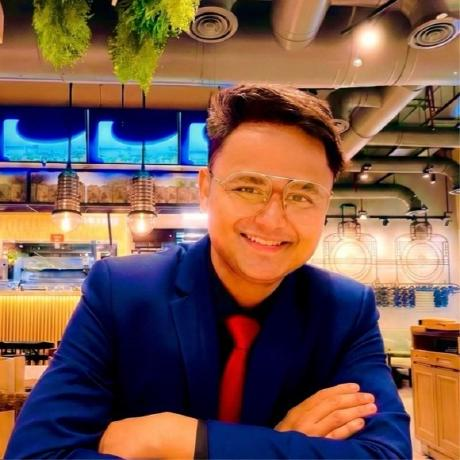
\includegraphics[width=1.9cm]{sarvesh-talele.jpg}};\end{scope}
      \draw[rule, line width=1pt] (4.4,0) circle (0.95cm);
      \node[below, font=\small\bfseries] at (4.4,-1.1) {Sarvesh Talele};
      \node[below, font=\tiny, text=muted] at (4.4,-1.5) {Mumbai, India};

      \node[font=\tiny, text=muted] at (2.2,-2.3) {Independent Research \quad$\cdot$\quad 2026};
    \end{tikzpicture}
  \end{center}
  \note{Greeting, then the one-line hook: a model has two memories, what it
  learned in training and what you put in the prompt, and this talk is about
  what happens when those two disagree. Do not name the framework yet. Twenty
  minutes, questions at the end. Target: 45 seconds on this slide.}
\end{frame}

% ============================== 2. HOOK ======================================
\begin{frame}{Start with a question}
  \vspace{0.5cm}
  \begin{center}
    {\Large You paste a document into a model's prompt.}\\[6mm]
    {\Large The document contradicts what the model learned.}\\[9mm]
    {\LARGE\bfseries\color{acquire} Which one wins?}
  \end{center}
  \vspace{0.6cm}
  \begin{center}\color{muted}\small
    Most of us assume the prompt wins. That assumption is what this talk tests.
  \end{center}
  \note{Ask it as a real question and pause for two seconds. Many in the room
  build retrieval systems on the assumption that context overrides the weights.
  Getting them to notice they hold that assumption is what makes the measurement
  land later. Target: 45 seconds.}
\end{frame}

% ============================== 3. PROBLEM ===================================
\begin{frame}{The field is fragmented}
  \begin{itemize}\setlength\itemsep{1.0em}
    \item Five research communities each own one part of how a model handles a fact:
      \begin{itemize}\setlength\itemsep{0.25em}
        \item retrieval-augmented generation \quad$\cdot$\quad knowledge editing
        \item continual learning \quad$\cdot$\quad context engineering \quad$\cdot$\quad agent memory
      \end{itemize}
    \item Each has its own benchmarks. Each passes them.
    \item A deployed system can pass all five and still fail, because nothing tests
          what happens \textbf{between} them.
  \end{itemize}
  \vspace{0.8em}
  \begin{center}
    \color{muted}Across 20 representative papers, median coverage is \textbf{two} of five stages.
  \end{center}
  \note{The audience knows all five fields. What is new is the claim that they
  are one system and nobody owns the joints. The median of two is the evidence
  for that claim, so state it plainly and move on rather than defending it here.
  Target: 90 seconds.}
\end{frame}

% ============================== 4. FRAMEWORK =================================
\begin{frame}{The framework: five stages}
  \begin{center}
  \small
  \begin{tabular}{@{}p{2.4cm}p{5.3cm}p{4.6cm}@{}}
    \toprule
    \textbf{Stage} & \textbf{What happens to the fact} & \textbf{Studied as} \\
    \midrule
    \textcolor{acquire}{$\blacksquare$}\ \textbf{Acquire}   & Training compresses a corpus into weights & Pre-training, fine-tuning \\[2pt]
    \textcolor{store}{$\blacksquare$}\ \textbf{Store}       & Weights, an external index, or both       & Parametric memory, vector stores \\[2pt]
    \textcolor{retrieve}{$\blacksquare$}\ \textbf{Retrieve} & Attention recalls, or a pipeline fetches  & Retrieval-augmented generation \\[2pt]
    \textcolor{update}{$\blacksquare$}\ \textbf{Update}     & The world changes; copies must follow     & Knowledge editing, continual learning \\[2pt]
    \textcolor{forget}{$\blacksquare$}\ \textbf{Forget}     & Removed on purpose, or lost by accident   & Unlearning, catastrophic forgetting \\
    \bottomrule
  \end{tabular}
  \end{center}
  \vspace{0.9em}
  \begin{center}
    The failure in this talk sits between
    \textcolor{retrieve}{\textbf{Retrieve}} and \textcolor{update}{\textbf{Update}}.
  \end{center}
  \note{This table is the contribution. Read the five stage names aloud so they
  are anchored, then land on the last line. The point to make: that boundary
  belongs to neither field beside it, which is exactly why it goes untested.
  Target: 2 minutes.}
\end{frame}

% ============================== 5. THE CASE ==================================
\begin{frame}{The probe}
  \vspace{0.3cm}
  \begin{itemize}\setlength\itemsep{0.9em}
    \item Take a fact the model certainly holds: the capital of France.
    \item Put a document in the prompt asserting a plausible substitute:
          \emph{the capital was relocated to Lyon}.
    \item Now the conflict exists \textbf{by construction}, for every model,
          whatever it was trained on and whenever.
  \end{itemize}
  \vspace{1.0em}
  \begin{center}
    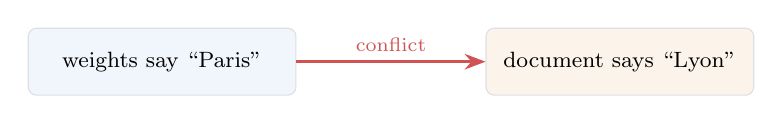
\begin{tikzpicture}[font=\footnotesize, node distance=0.35cm]
      \node[draw=rule, rounded corners=3pt, fill=acquire!8, minimum width=3.4cm, minimum height=0.85cm] (w) {weights say ``Paris''};
      \node[draw=rule, rounded corners=3pt, fill=retrieve!10, minimum width=3.4cm, minimum height=0.85cm, right=2.4cm of w] (d) {document says ``Lyon''};
      \draw[-{Stealth}, update, line width=1pt] (w) -- node[above, font=\scriptsize, text=update] {conflict} (d);
    \end{tikzpicture}
  \end{center}
  \note{The counterfactual is the whole methodological point and is worth
  labouring. A real-world update only creates a conflict for a model whose
  training predates it, so with six models of different vintages you cannot tell
  a model that deferred from one that never knew. Target: 75 seconds.}
\end{frame}

% ============================== 6. THE RESULT ================================
\begin{frame}{The measurement}
  \begin{center}
  \begin{tabular}{@{}lrrr@{}}
    \toprule
    \textbf{Model} & \textbf{Params} & \textbf{Holds it} & \textbf{Adopts the doc} \\
    \midrule
    GPT-2            & 124M  & 25.0\% & 50.0\% \\
    GPT-2 medium     & 355M  & 54.2\% & 43.6\% \\
    Qwen2.5-0.5B     & 494M  & 68.1\% & \textcolor{ok}{\textbf{91.8\%}} \\
    GPT-2 large      & 774M  & 79.2\% & 75.4\% \\
    TinyLlama-1.1B   & 1100M & 97.2\% & \textcolor{update}{\textbf{38.6\%}} \\
    Qwen2.5-1.5B     & 1540M & 98.6\% & 87.3\% \\
    \bottomrule
  \end{tabular}
  \end{center}
  \vspace{1.0em}
  \begin{itemize}\setlength\itemsep{0.7em}
    \item \textbf{864 forward passes.} Six models, 24 probes, three phrasings,
          with and without the document.
    \item Restricted to the \textbf{304} pairs where the model demonstrably held
          the fact, so a conflict actually existed.
  \end{itemize}
  \note{Let the third column land before saying anything. Holding the fact
  climbs straight down the column; adopting the document does not. If challenged
  on cherry-picking: the script is deterministic and in the repository.
  Target: 2 minutes.}
\end{frame}

% ============================== 7. SCALE DOES NOT FIX IT =====================
\begin{frame}{Scale buys knowledge, not deference}
  \vspace{0.4cm}
  \begin{center}
    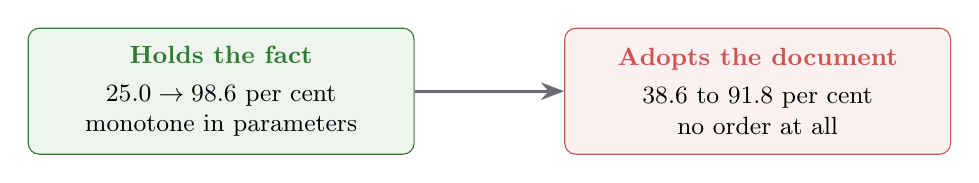
\begin{tikzpicture}[font=\small]
      \node[draw=ok, fill=ok!8, rounded corners=4pt, minimum width=4.9cm, minimum height=1.6cm, align=center] (k)
        {\textcolor{ok}{\textbf{Holds the fact}}\\[1mm] $25.0 \to 98.6$ per cent\\monotone in parameters};
      \node[draw=update, fill=update!8, rounded corners=4pt, minimum width=4.9cm, minimum height=1.6cm, align=center, right=1.9cm of k] (a)
        {\textcolor{update}{\textbf{Adopts the document}}\\[1mm] $38.6$ to $91.8$ per cent\\no order at all};
      \draw[-{Stealth}, line width=1.2pt, muted] (k) -- (a);
    \end{tikzpicture}
  \end{center}
  \vspace{1.0em}
  \begin{center}
    TinyLlama holds the fact \textbf{97.2\%} of the time and defers \textbf{least}
    of the six.\\
    Qwen2.5-0.5B, a third its size, defers \textbf{91.8\%}.
  \end{center}
  \note{This is the headline. A bigger model knows more and is not thereby more
  willing to be corrected. Family and training appear to matter more than size,
  though this design cannot separate them and the paper says so.
  Target: 90 seconds.}
\end{frame}

% ============================== 8. PHRASING ==================================
\begin{frame}{The wording moves it as much as the model does}
  \vspace{0.5cm}
  \begin{itemize}\setlength\itemsep{0.9em}
    \item Each probe is asked three ways, same question, different words.
    \item Across the three, the adoption rate has a median spread of
          \textbf{47.9} percentage points and a maximum of \textbf{87.5}.
    \item Qwen2.5-0.5B runs from \textbf{100.0\%} to \textbf{12.5\%} on the
          \emph{same 24 facts} with the \emph{same document}.
  \end{itemize}
  \vspace{1.2em}
  \begin{center}
    A single-phrasing result about knowledge conflict is reporting a property of
    the sentence\\ at least as much as a property of the model.
  \end{center}
  \note{This is the slide that makes the audience distrust every
  single-prompt result they have seen this year, including the earlier version
  of this one. Target: 75 seconds.}
\end{frame}

% ============================== 9. RANK ======================================
\begin{frame}{Probability is not an answer}
  \vspace{0.4cm}
  \begin{itemize}\setlength\itemsep{0.9em}
    \item Probability mass is spread over tens of thousands of tokens. An answer
          has only to be \textbf{ranked first}, not to be large.
    \item The in-context answer carries more than $0.10$ in \textbf{332} of the
          432 conditions with the document present.
    \item In \textbf{69} of those, \textbf{20.8\%}, it is \emph{still not} what
          the model says.
  \end{itemize}
  \vspace{1.2em}
  \begin{center}
    Recording the rank costs \textbf{one comparison} against the maximum,\\
    and it is the only quantity that matches what a deployed system emits.
  \end{center}
  \note{Slow down here. This is the methodological contribution and the next
  slide is the confession that motivates it. Target: 75 seconds.}
\end{frame}

% ============================== 10. THE CORRECTION ===========================
\begin{frame}{A correction to our own earlier report}
  \vspace{0.4cm}
  \begin{itemize}\setlength\itemsep{0.85em}
    \item An earlier version of this work reported that \textbf{no model} answers
          a drug-withdrawal probe correctly under any phrasing.
    \item \textbf{That claim was false.} The script behind it recorded only the
          \emph{surprisal} of the expected answer, never its rank, so it could
          not have tested the claim it was cited for.
    \item Re-run with rank recorded: \textbf{three of the six} rank the corrected
          answer first under two of three phrasings.
    \item A second defect was structural. Those probes were real-world updates,
          and the withdrawal predates every model's training data, so \textbf{no
          conflict existed to resist}.
  \end{itemize}
  \note{Say this plainly and do not soften it. Volunteering the error buys
  credibility for everything else, and a room that hears you correct yourself
  will believe the rest. Target: 90 seconds.}
\end{frame}

% ============================== 13. HONESTY ==================================
\begin{frame}{What is measured, and what is proposed}
  \vspace{0.4cm}
  \begin{center}
    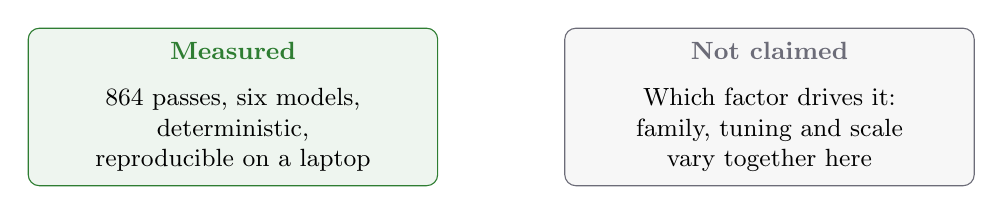
\begin{tikzpicture}[font=\small]
      \node[draw=ok, fill=ok!8, rounded corners=4pt, minimum width=5.2cm, minimum height=2.0cm, align=center] (m)
        {\textcolor{ok}{\textbf{Measured}}\\[2mm] 864 passes, six models,\\deterministic,\\reproducible on a laptop};
      \node[draw=muted, fill=black!3, rounded corners=4pt, minimum width=5.2cm, minimum height=2.0cm, align=center, right=1.6cm of m] (p)
        {\textcolor{muted}{\textbf{Not claimed}}\\[2mm] Which factor drives it:\\family, tuning and scale\\vary together here};
    \end{tikzpicture}
  \end{center}
  \vspace{0.9em}
  \begin{center}
    Every figure here is \textbf{generated} from the measurement, never typed.\\
    The earlier version quoted a number its own code had never produced.
  \end{center}
  \note{Say this before anyone asks. Volunteering the limitation buys credibility
  for everything else in the talk, and it removes the sharpest question a jury
  can put to you. Target: 60 seconds.}
\end{frame}

% ============================== 14. REPRODUCIBILITY ==========================
\begin{frame}{Check it yourself}
  \vspace{0.4cm}
  \begin{itemize}\setlength\itemsep{0.9em}
    \item Every number in this talk comes from \textbf{one deterministic script}.
          No sampling, identical digits on any machine.
    \item Six open models from 124M to 1.5B, float32 on CPU, so the digits do
          not depend on an accelerator's arithmetic.
    \item The demonstration runs GPT-2 \textbf{inside your browser}. Nothing you type
          leaves your laptop.
  \end{itemize}
  \vspace{1.2em}
  \begin{center}\footnotesize
    \textbf{Paper and code}\quad \href{https://github.com/Amey-Thakur/LLM-KNOWLEDGE-LIFECYCLE}{github.com/Amey-Thakur/LLM-KNOWLEDGE-LIFECYCLE}\\[2.5mm]
    \textbf{Live demonstration}\quad \href{https://huggingface.co/spaces/ameythakur/llm-knowledge-lifecycle}{huggingface.co/spaces/ameythakur/llm-knowledge-lifecycle}
  \end{center}
  \note{If there is a screen and a minute to spare, open the demo live and run
  a counterfactual probe. A measurement performed in front of the room is worth more
  than any slide. Target: 90 seconds, or 2 minutes with the live run.}
\end{frame}

% ============================== 15. WHAT NEXT ================================
\begin{frame}{What comes next}
  \begin{itemize}\setlength\itemsep{0.9em}
    \item \textbf{Which factor actually drives deference?} Family, instruction
          tuning and scale vary together across these six models, so the negative
          claim is supported and the positive one is not. Holding two fixed is the
          next experiment.
    \item \textbf{Does it hold above 1.5B?} Unknown. The non-monotonicity is
          evidence about this range, and 7B and above may behave differently.
    \item \textbf{Does reasoning-mode inference help?} Extended test-time compute
          should, in principle, resolve conflicts the forward pass cannot.
    \item \textbf{Multimodal.} A text prior overriding a contradicting image is the
          same failure in another modality.
  \end{itemize}
  % One line. At \small this note wraps into the footer band and runs across
  % the running title.
  \vspace{0.5em}
  \begin{center}\color{muted}\small
    Both answered, and both answers are largely negative.
  \end{center}
  \note{The first two bullets are results now, not plans, and the honest answer
  to both is close to a null. Say so plainly: the failure this paper names is
  not something the field will scale its way out of, and that is precisely why
  it needs an architectural fix rather than a bigger model. The full table is
  Section 8.6 of the paper. Target: 90 seconds.}
\end{frame}

% ============================== 16. SUMMARY ==================================
\begin{frame}{In three sentences}
  \vspace{1.0cm}
  \begin{itemize}\setlength\itemsep{1.3em}
    \item Five separate research fields are five stages of \textbf{one lifecycle},
          and systems fail at the boundaries nobody benchmarks.
    \item Whether a document beats a model's memory is \textbf{not a question of
          size}: holding a fact scales, deferring to a correction does not.
    \item And it has to be read at the \textbf{rank}, because probability and
          answer disagree one time in five.
  \end{itemize}
  \vspace{1.2em}
  \begin{center}
    
\begin{tikzpicture}
      \foreach \c/\n [count=\i from 0] in
        {acquire/Acquire, store/Store, retrieve/Retrieve, update/Update, forget/Forget}
        \node[fill=\c, text=white, font=\scriptsize\bfseries, rounded corners=2pt,
              minimum width=1.9cm, minimum height=0.55cm] at (\i*2.05, 0) {\n};
    \end{tikzpicture}
  \end{center}
  \note{If you are running short, this slide can carry the last three minutes on
  its own. Say each bullet once, without elaborating, then go to questions.
  Target: 60 seconds.}
\end{frame}

% ============================== 17. THANK YOU ================================
\begin{frame}[plain]
  \vspace{1.3cm}
  \begin{center}
    {\Large\bfseries Thank you}\\[3mm]
    {\color{muted}\small Questions}\\[10mm]

    \begin{tikzpicture}
      \begin{scope}\clip (0,0) circle (0.8cm);
        \node at (0,0) {
\includegraphics[width=1.6cm]{amey-thakur.jpg}};\end{scope}
      \draw[rule, line width=1pt] (0,0) circle (0.8cm);
      \node[below, font=\footnotesize\bfseries] at (0,-0.95) {Amey Thakur};
      \node[below, font=\tiny, text=muted] at (0,-1.3) {\href{mailto:ameythakur20@gmail.com}{ameythakur20@gmail.com}};

      \begin{scope}\clip (5.2,0) circle (0.8cm);
        \node at (5.2,0) {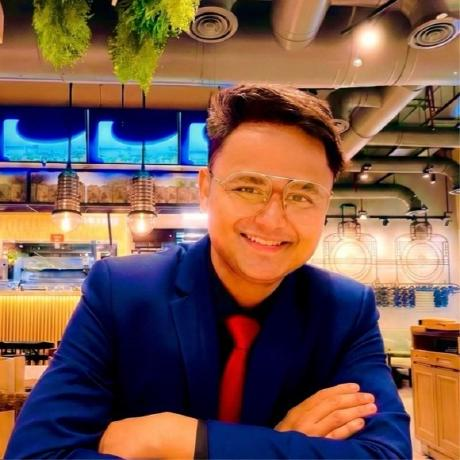
\includegraphics[width=1.6cm]{sarvesh-talele.jpg}};\end{scope}
      \draw[rule, line width=1pt] (5.2,0) circle (0.8cm);
      \node[below, font=\footnotesize\bfseries] at (5.2,-0.95) {Sarvesh Talele};
      \node[below, font=\tiny, text=muted] at (5.2,-1.3) {\href{mailto:talelesarvesh@gmail.com}{talelesarvesh@gmail.com}};
    \end{tikzpicture}\\[7mm]

    {\scriptsize\href{https://github.com/Amey-Thakur/LLM-KNOWLEDGE-LIFECYCLE}{github.com/Amey-Thakur/LLM-KNOWLEDGE-LIFECYCLE}}
  \end{center}
  \note{Leave this slide up for the whole question period so the contact details
  and repository stay visible. The backup slide follows if a question needs it.}
\end{frame}

% ============================== 18. BACKUP ===================================
\begin{frame}{Backup: anticipated questions}
  \vspace{0.2cm}
  \small
  \begin{itemize}\setlength\itemsep{0.75em}
    \item \textbf{Why models this small?} Fully open, and the whole measurement
          reruns on a laptop in twenty minutes. The claim is about this range and
          says so; 7B and above is untested.
    \item \textbf{Is this just hallucination?} No. The document is placed in the
          prompt by construction, so nothing was lost in retrieval. What fails is
          the step after it.
    \item \textbf{Aren't counterfactual documents unfair?} They are a different
          case from a deployed system, where the document is true and the memory
          is stale. They buy freedom from the training-cutoff confound, and a
          model that defers here may be deferring to misinformation too. Both are
          in the limitations.
    \item \textbf{Why only capitals?} It controls for question type, at the cost
          of saying nothing about numeric, temporal or causal facts.
    \item \textbf{Why does the earlier claim appear at all?} Because it was
          published. Correcting it on the record is cheaper than letting someone
          else find it.
  \end{itemize}
  \note{Do not show this slide unless a question calls for it. Knowing it is
  there is what keeps you calm during questions.}
\end{frame}

\end{document}
